\documentclass[]{article}

\usepackage{xargs} 
\usepackage[colorinlistoftodos,prependcaption,textsize=tiny]{todonotes}
\newcommandx{\unsure}[2][1=]{\todo[linecolor=red,backgroundcolor=red!25,bordercolor=red,#1]{#2}}
\newcommandx{\change}[2][1=]{\todo[linecolor=blue,backgroundcolor=blue!25,bordercolor=blue,#1]{#2}}
\newcommandx{\info}[2][1=]{\todo[linecolor=OliveGreen,backgroundcolor=OliveGreen!25,bordercolor=OliveGreen,#1]{#2}}
\newcommandx{\improvement}[2][1=]{\todo[linecolor=purple,backgroundcolor=purple!25,bordercolor=purple,#1]{#2}}
\newcommandx{\thiswillnotshow}[2][1=]{\todo[disable,#1]{#2}}

\usepackage{enumitem}
\usepackage{multicol}

\usepackage{graphicx}
\usepackage{caption}
\usepackage{subcaption}

%opening
\title{}
\author{}

\begin{document}

\maketitle

\begin{abstract}

\end{abstract}

\section{Introduction}

Multitouch gestural interfaces, like those found on tablets and smartphones, offer the possibility of a very direct user experience, especially compared to the Windows, Icons, Mouse, Pointer (WIMP) interface design. 
Rather than, for example, using an arrow key to scroll in a document, the user can drag the document directly, as though they were sliding a long piece of paper on table. 

This directness is a hallmark of what has come to be called Natural User Interfaces, or NUI. 
A natural user interface is one that allows the user to re-use existing skills and natural motions to interact directly with content \cite{blakeNUIWin}. 
In practice, this means that the elements of the interaction are actions such as pointing and other gestures, drawing with a pen, speech, gaze, and so forth, rather than computer-specific interface devices. 
By way of contrast, the command line interface is defined in terms of typing with some form of keyboard, and the graphic user interface is (in most cases), defined in terms of mouse actions. 

However, as the number of operations the user wishes to perform increases, the limitations of multitouch screens become more apparent. 
Screens are flat, and so only afford 2-dimensional gestures, such as dragging, poking, and tapping. 
Even if the screen depicts a 2-dimensional projection of a 3-dimensional world, operations that would make sense in the 3D world, such as grasping, have to be mapped to the 2-dimensional space of operations to be performed. 
Typically, the gestures that the user uses to perform the available operations are chosen by the interface developer, and the user is trained to perform them, possibly by a short tutorial program \cite{wobbrock2009user, vanacken2008ghosts, freeman2009shadowguides}. 

Unfortunately, the use of screens with interactions inspired by the affordances of physical objects leads to the user having to decide between ``natural'' skills and motions, which are used on physical objects, and the skills and actions used with screens: single-point dragging and clicking. 
Most users understand that they are looking at pictures of things on a screen, and so default to single-point interactions \cite{vanacken2008ghosts}

In this paper, we attempt to discover the gestures that users would choose themselves, based on their own thinking about the interface and, likely, their own past experience with computer technology such as tablets, smartphones, and video games. 

This work is an extension of previous work that used a similar process to discover user interface gestures for single or small groups of robots. We extend this method to larger groups of robots, in an attempt to discover if the gestures that users select vary with the number of robots available. \todo{can't say much here without results}. 

\section{Related Work}

Previous attempts to build user interface gesture sets can be broadly separated into two classes, those that attempt to build a general gesture set, and those that attempt to build a gesture set to be used for a specific task. 
General gesture sets would be for operations such as the cut/copy/paste editing metaphors, which show up in word processing, image editing, and other productivity applications. 
These operations act in related but differing ways, depending on their context, but are invoked in the same way across applications and even across operating systems. 
Task-specific gestures are for operations such as flying through a 3D rendering of an architectural space, or transposing cells in a spreadsheet. 
While somewhat intuitive gestures may exist for both operations, the operation is tightly bound to the task at hand, and the gestures would likely be different. 

Yao, Fernando, and Wang develop a set of task-specific gestures for urban planning from the required functionality of the interface and paper prototyping on a table \cite{yao2012multi}. 
The gestures were collected by placing a map on the table, and asking users to perform the gestures they would use to access the required functions. 
The resulting interface is modal, depending on the user's desired method of interaction, different gestures are available. 
The interface also permits the combination of some gestures, such as panning or rotating the map while zooming in or out as well. 

Micire \textit{et al}. develops a taxonomy of user gestures for control of both robots and of the interface to control them \cite{Micire:2009:ANG:1731903.1731912}. 
The interface control gestures are for actions such as zooming in on the content of the screen or panning around a map. 
Individual users chose a variety of gestures to perform the tasks, but for almost all types of tasks, having two gestures available to perform it would be sufficient to cover 60\% of the users. 
It was also noted that the gestures that users use are informed by their previous experience both with WIMP interfaces and with touch-screen technology. 
Since smartphones are a common multitouch interaction device, it would be expected that smartphone users expectations of multitouch interaction would be informed by their phones. 
Micire \textit{et al}. confirmed this, finding that iPhone owners used significantly more pinch gestures than participants with no iPhone experience. 

At a more general level, Wobbrock, Morris, and Wilson use an interesting technique to elicit gestures from non-technical users \cite{wobbrock2009user}.
The user is shown the \textit{effect} of a command, and then asked to perform the gesture that \textit{caused} that effect. 
The users were asked to think aloud, in order to understand their cognition about the system and gestures, in addition to their behaviour. 
The experiment used 27 commands: move a little, move a lot, select single, rotate, shrink, delete, enlarge, pan, close, zoom in, zoom out, select group, open, duplicate, previous, next, insert, maximize, paste, minimize, cut, accept, reject, access menu, help, task switch, and undo (listed in order of complexity as ranked by Wobbrock \textit{et al}).
Many of these commands are related to window managers, or occur in some form in multiple applications, such as the cut/copy/paste metaphors. 
As a result, this general gesture set could be used in a gestural window manager or operating system interface, while the gesture sets developed by Micire \textit{et al}; Yao, Fernando, and Wang; or in this work are all intended to provide a more precise set of meanings for a single application and task. 

\section{Experiment Setup}

\todo{put a picture of the experiment setup here}

The multitouch user interface device used in this experiment is a 3M \todo{Exact model here} screen. 
This screen can track up to 20 simultaneous points, but reports only points, rather than shapes or areas of contact. \todo{pressure information? I think I had this in my initial drawing scripts}

Users were seated in front of the interface and read a script describing the system and the experiment. The user interface displayed alternating slides of instructions to the user, such as "Move the robots to area A" and interface screens for them to interact with. 
The interface did not visibly respond to user contact or move the robots depicted on it.
In this regard, it more closely resembles the paper prototypes of the User-centered Design process \todo{cite} than a fully functional interface.

While the user interacted with the touch screen, their touches and the positions of their hands were recorded by the computer connected to the screen and by the video cameras. 
One video camera was placed high, looking down at the screen, to track where the user's hand position over the screen. 
The other video camera was placed in front of the screen at a low angle, in order to observe whether the user's hands were touching the screen, or moving above it. 
In addition to screen contacts and video, users were asked to think aloud about their actions and the things they said were recorded as well. 

The software used to record all of this information is ROS, the Robot Operating System \todo{cite}. 
ROS was developed as a message-passing framework for connecting modular programs on a robot \todo{explain better when not tired}. 
It may seem unusual to use a framework intended for operating robots as a recording program for collecting experiment data, but ROS provides a utility called rosbag that records some or all of the messages emitted by the robot's sensors in a ``bag'' file. 
In this case, the cameras, microphone, and UI application are the ``sensors'' for rosbag to record.
A ROS launch file starts multiple ROS nodes to record image data from the cameras, audio from the microphone, and touch events and screen updates from the UI.
ROS also provides tools for manipulating bag files, and playing them back. 
All of the data in the file is timestamped, so it plays back with the audio, video, and UI interactions all accurately synchronized. 
Because all of the data is treated as standard ROS message types, it is relatively easy to write custom processors for the recorded data.
For example, a node was written that accepts the replayed UI screen changes and touch events, and renders them as a stream of ROS image messages showing the contact points overlaid on the UI screen. 

\subsection{Experiment Conditions}

Users were given tasks in one of five conditions, varying by how many robots were in each condition. 
The conditions consisted of 1-2 robots, 10 robots, 100 robots, 1000 robots, or an unknown number of robots, represented by a cloud. 
For each condition, the user was requested to perform a sequence of tasks. 
The exact number of tasks varied between conditions due to some tasks not making sense with the number of robots involved. 

\begin{tabular}{l|l|l|l|l|l}
& 1 & 10 & 100 & 1000 & Unknown \\
Move to area A & x & x & x & x & x\\
Move to area A with a wall & x & x & x & x & x \\
Stop the robots & x & x & x & x & x\\
Divide around an obstacle & & x & x & x & x \\
Orange to B, red to A & x & x & x & x & x \\
Orange to A, red to B & x & x & x & x & x \\
Orange to A, red to B (mixed) & x & x & x & x & x \\
Divide group & x & x & x & x & x \\
Merge groups & & x & x & x & x \\
Form a line & & x & x & x & x \\
Form a square & & x & x & x & x \\
Move the crate to area A & x & x & x & x & x \\
Move the crate to area A (dispersed) & x & x & x & x & x\\
Mark defective robot & x & x & x & x & \\
Remove defective robot & x & x & x & x &  \\
Patrol the screen border & x & x & x & x & x \\
Patrol area A & x & x & x & x & x \\
Disperse over screen & x & x & x & x & x \\
\end{tabular}

The individual robot case is lacking the tasks that do not make sense for a single robot. A single robot cannot, for example, divide around an obstacle or form a square. 
The ``Merge groups" task was left out of the single robot case because of the potential for confusion when referring to a ``group'' of one robot as a group. 

The unknown number of robots condition has the same tasks as the 10, 100, and 1000 robot cases, except for the ``Mark defective robot" and ``Remove defective robot" task. 
Without UI elements that represent individual robots, the user cannot take any actions that refer to a specific robot. 


\section{Analysis}

User gestures were coded using a methodology adopted from the social sciences, Grounded Theory \todo{cite}.
Grounded Theory is an iterative process, where the data are first coded at a very fine-grained level, and then the resulting coded elements are compared to each other to try to determine their qualities, similarities, and differences. 
Codes can be consolidated or divided until repeated passes of coding and comparison no longer alter the emerging structure of the coding scheme. 
During each iteration of coding and comparison, the coder makes memos as well, describing the links they see between related coded elements and higher-level abstractions that relate the elements. 
These memos are eventually written up as the social scientific theory, which is believed to be grounded in the data because it arises from the coding process. 

We had NNN coders, and performed NNN \todo{I hope this is "2" at most} passes through the data.
Coding based on Mark's paper for initial pass, plus open coding to encompass anything that that didn't cover. 
After the first pass of coding, the coders met to compare memos and coding elements. During this meeting, we created a code book based on the codes that each coder developed. All of the video was then recoded using the common codebook. 



[DATA INTENSIFIES]
 
Some people take the directions on the slides very literally. 
For example, users who had been solely using the touch interface read the slides that instructed "Tell the robots to form a line" to indicate that they should speak the words "Form a line", addressed to the robots.

People who didn't otherwise want voice commands would use them for the task of stopping the robots. 
Since this task assumes the robots are already moving towards a goal, attempts to interact with all of them while they are moving could be difficult. 

For the task of removing the defective robot, the location selected for it to be removed to was usually either a corner, a ``recycle bin" or similar disposal area, or off the edge of the screen. This use of the area beyond the screen for placement of deleted or rejected things parallels that seen by Wobbrock \textit{et al}.

\subsection{Participant Demographics}

The experiment had 50 participants, 10 per condition. 

\section{Conclusions}

In future, it might be interesting to repeat this work with a condition that does not display the robots in the user interface at all. 
We expect that for conditions such as the ``move the crate'' tasks, the user would simply indicate the crate should move to area A, without concern for which robots perform the moving. 
However, such an interface would not afford indicating particular robots or groups, so tasks such as dividing the robots around an obstacle may become difficult to perform. 

\bibliography{../proposal/swarm.bib}
\bibliographystyle{apalike}

\section{Appendix of all Test Slides}
\begin{figure}
	\centering
	\begin{subfigure}{0.42\textwidth}
		\centering
		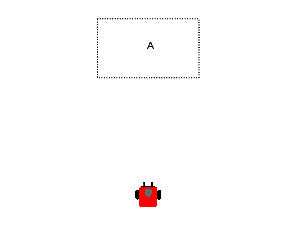
\includegraphics[width=\linewidth]{slide_images/Swarm_Robot_Control_-_Single_Robot_0003.png}
		\caption{Move to A}
		\label{fig:sub1}
	\end{subfigure}%
	\begin{subfigure}{0.42\textwidth}
		\centering
		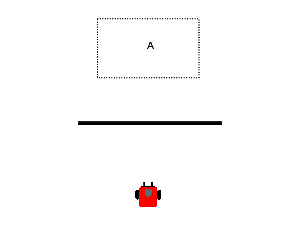
\includegraphics[width=\linewidth]{slide_images/Swarm_Robot_Control_-_Single_Robot_0005.png}
		\caption{Move to A with wall}
		\label{fig:sub2}
	\end{subfigure}
	\begin{subfigure}{0.42\textwidth}
		\centering
		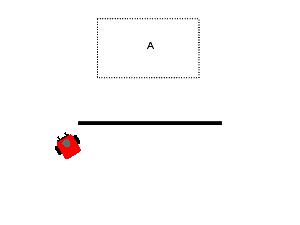
\includegraphics[width=\linewidth]{slide_images/Swarm_Robot_Control_-_Single_Robot_0007.png}
		\caption{Stop the robot}
		\label{fig:sub1}
	\end{subfigure}%
	\begin{subfigure}{0.42\textwidth}
		\centering
		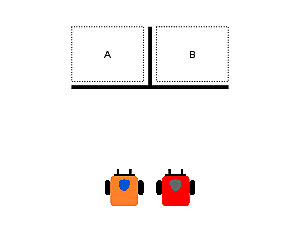
\includegraphics[width=\linewidth]{slide_images/Swarm_Robot_Control_-_Single_Robot_0009.png}
		\caption{Orange to B, Red to A}
		\label{fig:sub2}
	\end{subfigure}
	\begin{subfigure}{0.42\textwidth}
		\centering
		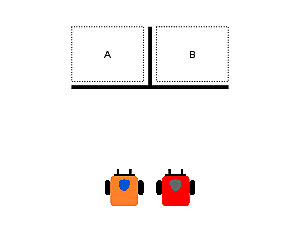
\includegraphics[width=\linewidth]{slide_images/Swarm_Robot_Control_-_Single_Robot_0011.png}
		\caption{Orange to A, Red to B}
		\label{fig:sub1}
	\end{subfigure}%
	\begin{subfigure}{0.42\textwidth}
		\centering
		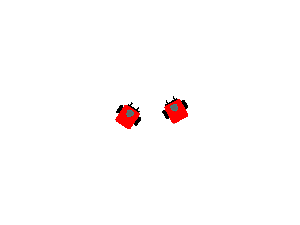
\includegraphics[width=\linewidth]{slide_images/Swarm_Robot_Control_-_Single_Robot_0013.png}
		\caption{Divide group}
		\label{fig:sub2}
	\end{subfigure}
	\begin{subfigure}{0.42\textwidth}
		\centering
		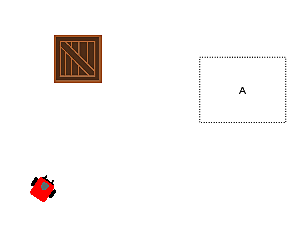
\includegraphics[width=\linewidth]{slide_images/Swarm_Robot_Control_-_Single_Robot_0015.png}
		\caption{Move the crate to A}
		\label{fig:sub1}
	\end{subfigure}%
	\begin{subfigure}{0.42\textwidth}
		\centering
		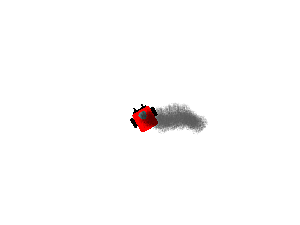
\includegraphics[width=\linewidth]{slide_images/Swarm_Robot_Control_-_Single_Robot_0017.png}
		\caption{Mark defective robot}
		\label{fig:sub2}
	\end{subfigure}
	\label{fig:single_robot_slides}
\end{figure}


\begin{figure}
	\ContinuedFloat
	\centering
	\begin{subfigure}{0.42\textwidth}
		\centering
		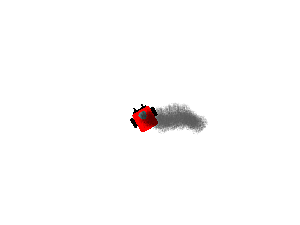
\includegraphics[width=\linewidth]{slide_images/Swarm_Robot_Control_-_Single_Robot_0019.png}
		\caption{Remove defective robot}
		\label{fig:sub1}
	\end{subfigure}%
	\begin{subfigure}{0.42\textwidth}
		\centering
		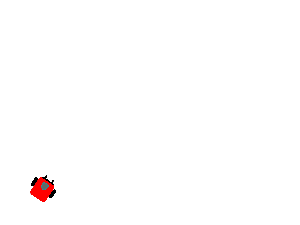
\includegraphics[width=\linewidth]{slide_images/Swarm_Robot_Control_-_Single_Robot_0021.png}
		\caption{Patrol the screen border}
		\label{fig:sub2}
	\end{subfigure}
	\begin{subfigure}{0.42\textwidth}
		\centering
		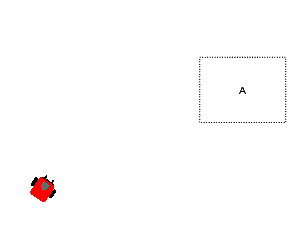
\includegraphics[width=\linewidth]{slide_images/Swarm_Robot_Control_-_Single_Robot_0023.png}
		\caption{Patrol area A}
		\label{fig:sub1}
	\end{subfigure}
	\label{fig:single_robot_slides_pt2}
\end{figure}


\begin{figure}
	\centering
	\begin{subfigure}{0.42\textwidth}
		\centering
		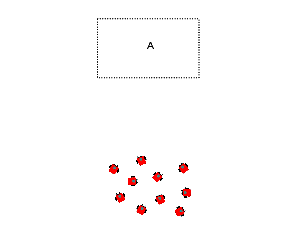
\includegraphics[width=\linewidth]{slide_images/Swarm_Robot_Control_-_10_Robot_0003.png}
		\caption{Move to A}
		\label{fig:sub1}
	\end{subfigure}%
	\begin{subfigure}{0.42\textwidth}
		\centering
		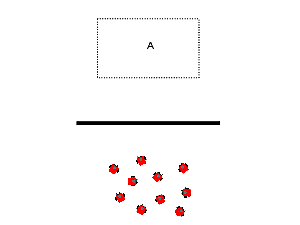
\includegraphics[width=\linewidth]{slide_images/Swarm_Robot_Control_-_10_Robot_0005.png}
		\caption{Move to A with wall}
		\label{fig:sub2}
	\end{subfigure}
	\begin{subfigure}{0.42\textwidth}
		\centering
		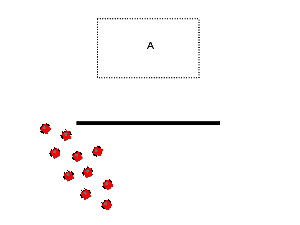
\includegraphics[width=\linewidth]{slide_images/Swarm_Robot_Control_-_10_Robot_0007.png}
		\caption{Stop the robots}
		\label{fig:sub1}
	\end{subfigure}%
	\begin{subfigure}{0.42\textwidth}
		\centering
		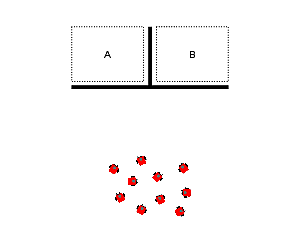
\includegraphics[width=\linewidth]{slide_images/Swarm_Robot_Control_-_10_Robot_0009.png}
		\caption{Divide around obstacle}
		\label{fig:sub2}
	\end{subfigure}
	\begin{subfigure}{0.42\textwidth}
		\centering
		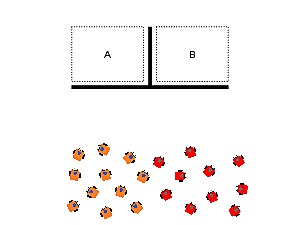
\includegraphics[width=\linewidth]{slide_images/Swarm_Robot_Control_-_10_Robot_0011.png}
		\caption{Orange to B, Red to A}
		\label{fig:sub1}
	\end{subfigure}%
	\begin{subfigure}{0.42\textwidth}
		\centering
		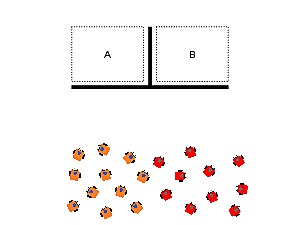
\includegraphics[width=\linewidth]{slide_images/Swarm_Robot_Control_-_10_Robot_0013.png}
		\caption{Orange to A, Red to B}
		\label{fig:sub2}
	\end{subfigure}
	\begin{subfigure}{0.42\textwidth}
		\centering
		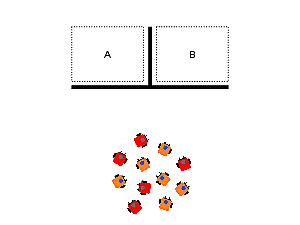
\includegraphics[width=\linewidth]{slide_images/Swarm_Robot_Control_-_10_Robot_0015.png}
		\caption{Orange to A, Red to B}
		\label{fig:sub1}
	\end{subfigure}%
	\begin{subfigure}{0.42\textwidth}
		\centering
		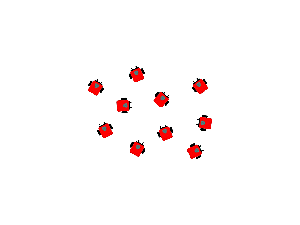
\includegraphics[width=\linewidth]{slide_images/Swarm_Robot_Control_-_10_Robot_0017.png}
		\caption{Divide group}
		\label{fig:sub2}
	\end{subfigure}
\end{figure}
	
	
\begin{figure}
	\ContinuedFloat
	\centering		
	\begin{subfigure}{0.42\textwidth}
		\centering
		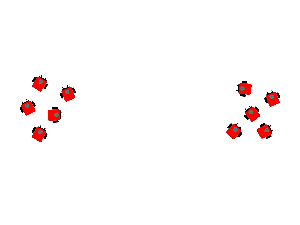
\includegraphics[width=\linewidth]{slide_images/Swarm_Robot_Control_-_10_Robot_0019.png}
		\caption{Combine groups}
		\label{fig:sub1}
	\end{subfigure}%
	\begin{subfigure}{0.42\textwidth}
		\centering
		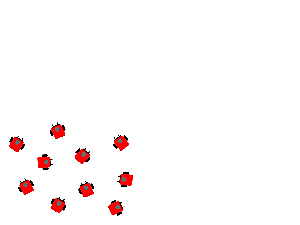
\includegraphics[width=\linewidth]{slide_images/Swarm_Robot_Control_-_10_Robot_0021.png}
		\caption{}
		\label{fig:sub2}
	\end{subfigure}
	\begin{subfigure}{0.42\textwidth}
		\centering
		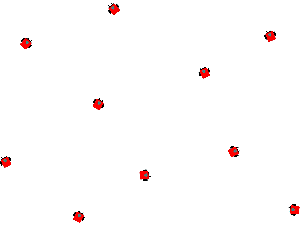
\includegraphics[width=\linewidth]{slide_images/Swarm_Robot_Control_-_10_Robot_0023.png}
		\caption{}
		\label{fig:sub1}
	\end{subfigure}%
	\begin{subfigure}{0.42\textwidth}
		\centering
		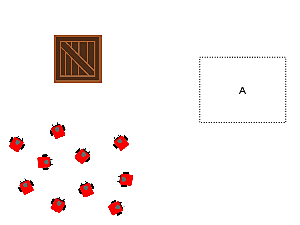
\includegraphics[width=\linewidth]{slide_images/Swarm_Robot_Control_-_10_Robot_0025.png}
		\caption{Orange to A, Red to B}
		\label{fig:sub1}
	\end{subfigure}
	\begin{subfigure}{0.42\textwidth}
		\centering
		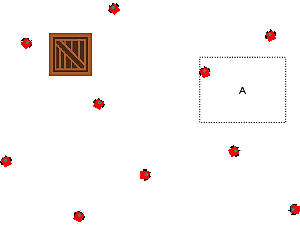
\includegraphics[width=\linewidth]{slide_images/Swarm_Robot_Control_-_10_Robot_0027.png}
		\caption{Divide group}
		\label{fig:sub2}
	\end{subfigure}%
	\begin{subfigure}{0.42\textwidth}
		\centering
		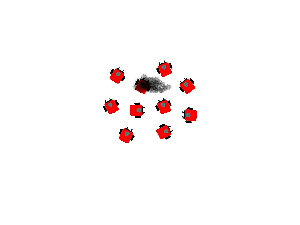
\includegraphics[width=\linewidth]{slide_images/Swarm_Robot_Control_-_10_Robot_0029.png}
		\caption{Combine groups}
		\label{fig:sub1}
	\end{subfigure}
	\begin{subfigure}{0.42\textwidth}
		\centering
		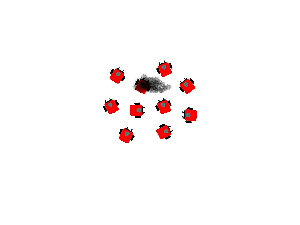
\includegraphics[width=\linewidth]{slide_images/Swarm_Robot_Control_-_10_Robot_0031.png}
		\caption{Form a line}
		\label{fig:sub2}
	\end{subfigure}%
	\begin{subfigure}{0.42\textwidth}
		\centering
		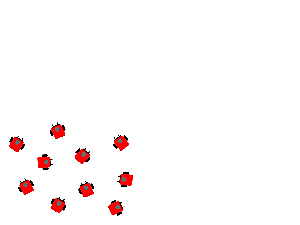
\includegraphics[width=\linewidth]{slide_images/Swarm_Robot_Control_-_10_Robot_0033.png}
		\caption{Form a square}
		\label{fig:sub1}
	\end{subfigure}
\end{figure}
	
	
\begin{figure}
	\ContinuedFloat
	\centering	
	\begin{subfigure}{0.42\textwidth}
		\centering
		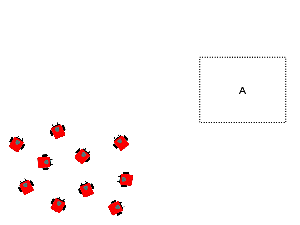
\includegraphics[width=\linewidth]{slide_images/Swarm_Robot_Control_-_10_Robot_0035.png}
		\caption{Move the crate to A}
		\label{fig:sub1}
	\end{subfigure}%
	\begin{subfigure}{0.42\textwidth}
		\centering
		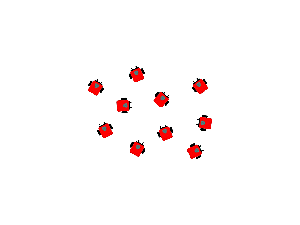
\includegraphics[width=\linewidth]{slide_images/Swarm_Robot_Control_-_10_Robot_0037.png}
		\caption{Move the crate to A}
		\label{fig:sub2}
	\end{subfigure}
	\label{fig:10_robot_slides}
\end{figure}

\begin{figure}
	\centering
	\begin{subfigure}{0.42\textwidth}
		\centering
		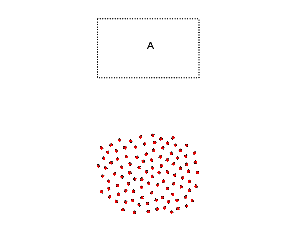
\includegraphics[width=\linewidth]{slide_images/Swarm_Robot_Control_-_100_Robot_0003.png}
		\caption{Move to A}
		\label{fig:sub1}
	\end{subfigure}%
	\begin{subfigure}{0.42\textwidth}
		\centering
		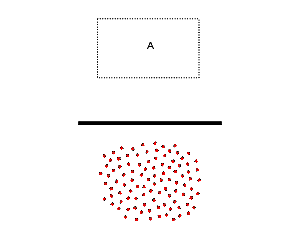
\includegraphics[width=\linewidth]{slide_images/Swarm_Robot_Control_-_100_Robot_0005.png}
		\caption{Move to A with wall}
		\label{fig:sub2}
	\end{subfigure}
	\begin{subfigure}{0.42\textwidth}
		\centering
		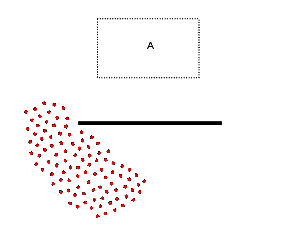
\includegraphics[width=\linewidth]{slide_images/Swarm_Robot_Control_-_100_Robot_0007.png}
		\caption{Stop the robots}
		\label{fig:sub1}
	\end{subfigure}%
	\begin{subfigure}{0.42\textwidth}
		\centering
		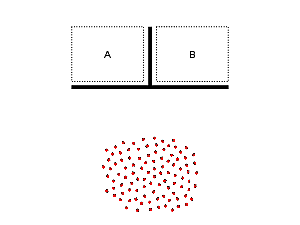
\includegraphics[width=\linewidth]{slide_images/Swarm_Robot_Control_-_100_Robot_0009.png}
		\caption{Divide around obstacle}
		\label{fig:sub2}
	\end{subfigure}
	\begin{subfigure}{0.42\textwidth}
		\centering
		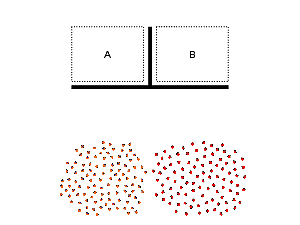
\includegraphics[width=\linewidth]{slide_images/Swarm_Robot_Control_-_100_Robot_0011.png}
		\caption{Orange to B, Red to A}
		\label{fig:sub1}
	\end{subfigure}%
	\begin{subfigure}{0.42\textwidth}
		\centering
		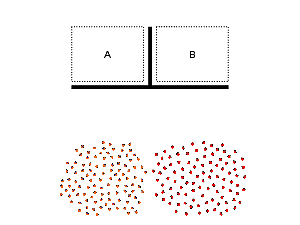
\includegraphics[width=\linewidth]{slide_images/Swarm_Robot_Control_-_100_Robot_0013.png}
		\caption{Orange to A, Red to B}
		\label{fig:sub2}
	\end{subfigure}
	\begin{subfigure}{0.42\textwidth}
		\centering
		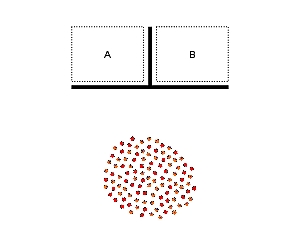
\includegraphics[width=\linewidth]{slide_images/Swarm_Robot_Control_-_100_Robot_0015.png}
		\caption{Orange to A, Red to B}
		\label{fig:sub1}
	\end{subfigure}%
	\begin{subfigure}{0.42\textwidth}
		\centering
		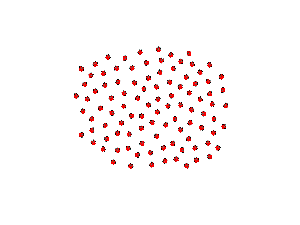
\includegraphics[width=\linewidth]{slide_images/Swarm_Robot_Control_-_100_Robot_0017.png}
		\caption{Divide group}
		\label{fig:sub2}
	\end{subfigure}
\end{figure}
\begin{figure}
	\ContinuedFloat
	\centering
	\begin{subfigure}{0.42\textwidth}
		\centering
		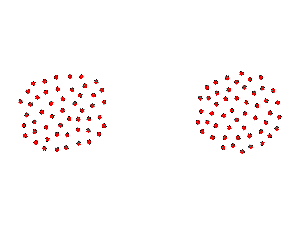
\includegraphics[width=\linewidth]{slide_images/Swarm_Robot_Control_-_100_Robot_0019.png}
		\caption{Combine groups}
		\label{fig:sub1}
	\end{subfigure}%
	\begin{subfigure}{0.42\textwidth}
		\centering
		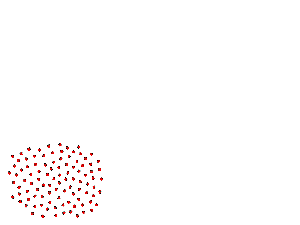
\includegraphics[width=\linewidth]{slide_images/Swarm_Robot_Control_-_100_Robot_0021.png}
		\caption{Form a line}
		\label{fig:sub2}
	\end{subfigure}
	\begin{subfigure}{0.42\textwidth}
		\centering
		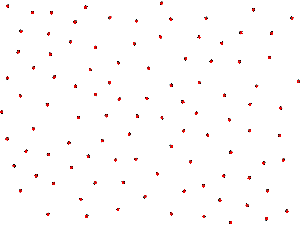
\includegraphics[width=\linewidth]{slide_images/Swarm_Robot_Control_-_100_Robot_0023.png}
		\caption{Form a square}
		\label{fig:sub1}
	\end{subfigure}%
	\begin{subfigure}{0.42\textwidth}
		\centering
		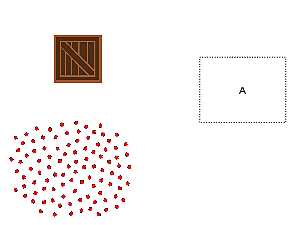
\includegraphics[width=\linewidth]{slide_images/Swarm_Robot_Control_-_100_Robot_0025.png}
		\caption{Move the crate to area A}
		\label{fig:sub1}
	\end{subfigure}
	\begin{subfigure}{0.42\textwidth}
		\centering
		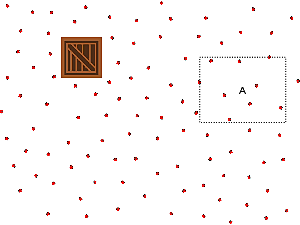
\includegraphics[width=\linewidth]{slide_images/Swarm_Robot_Control_-_100_Robot_0027.png}
		\caption{Move the crate to area A}
		\label{fig:sub2}
	\end{subfigure}%
	\begin{subfigure}{0.42\textwidth}
		\centering
		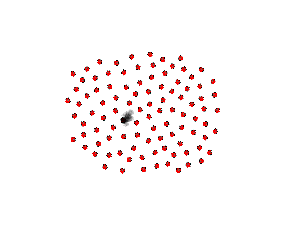
\includegraphics[width=\linewidth]{slide_images/Swarm_Robot_Control_-_100_Robot_0029.png}
		\caption{Mark defective robot}
		\label{fig:sub1}
	\end{subfigure}
	\begin{subfigure}{0.42\textwidth}
		\centering
		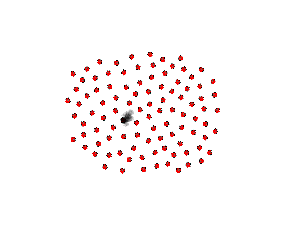
\includegraphics[width=\linewidth]{slide_images/Swarm_Robot_Control_-_100_Robot_0031.png}
		\caption{Remove defective robot}
		\label{fig:sub2}
	\end{subfigure}%
	\begin{subfigure}{0.42\textwidth}
		\centering
		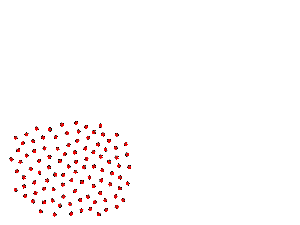
\includegraphics[width=\linewidth]{slide_images/Swarm_Robot_Control_-_100_Robot_0033.png}
		\caption{Patrol the screen border}
		\label{fig:sub1}
	\end{subfigure}
\end{figure}
\begin{figure}
	\ContinuedFloat
	\centering	
		\begin{subfigure}{0.42\textwidth}
		\centering
		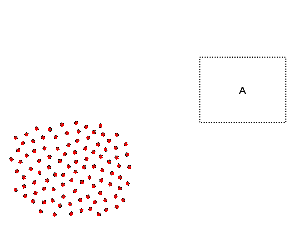
\includegraphics[width=\linewidth]{slide_images/Swarm_Robot_Control_-_100_Robot_0035.png}
		\caption{Patrol area A}
		\label{fig:sub1}
	\end{subfigure}%
	\begin{subfigure}{0.42\textwidth}
		\centering
		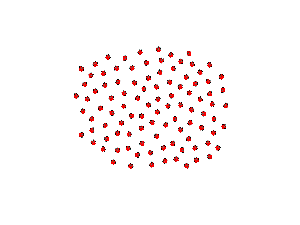
\includegraphics[width=\linewidth]{slide_images/Swarm_Robot_Control_-_100_Robot_0037.png}
		\caption{Disperse over screen}
		\label{fig:sub2}
	\end{subfigure}
	\label{fig:100_robot_slides}
\end{figure}


\begin{figure}
	\centering
	\begin{subfigure}{0.42\textwidth}
		\centering
		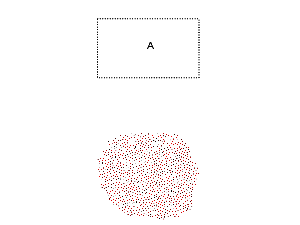
\includegraphics[width=\linewidth]{slide_images/Swarm_Robot_Control_-_1000_Robot_0003.png}
		\caption{Move to A}
		\label{fig:sub1}
	\end{subfigure}%
	\begin{subfigure}{0.42\textwidth}
		\centering
		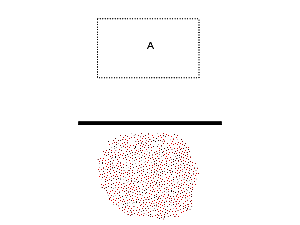
\includegraphics[width=\linewidth]{slide_images/Swarm_Robot_Control_-_1000_Robot_0005.png}
		\caption{Move to A with wall}
		\label{fig:sub2}
	\end{subfigure}
	\begin{subfigure}{0.42\textwidth}
		\centering
		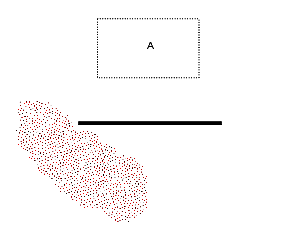
\includegraphics[width=\linewidth]{slide_images/Swarm_Robot_Control_-_1000_Robot_0007.png}
		\caption{Stop the robots}
		\label{fig:sub1}
	\end{subfigure}%
	\begin{subfigure}{0.42\textwidth}
		\centering
		\includegraphics[width=\linewidth]{slide_images/Swarm_Robot_Control_-_1000_Robot_0009.png}
		\caption{Divide around obstacle}
		\label{fig:sub2}
	\end{subfigure}
	\begin{subfigure}{0.42\textwidth}
		\centering
		\includegraphics[width=\linewidth]{slide_images/Swarm_Robot_Control_-_1000_Robot_0011.png}
		\caption{Orange to B, Red to A}
		\label{fig:sub1}
	\end{subfigure}%
	\begin{subfigure}{0.42\textwidth}
		\centering
		\includegraphics[width=\linewidth]{slide_images/Swarm_Robot_Control_-_1000_Robot_0013.png}
		\caption{Orange to A, Red to B}
		\label{fig:sub2}
	\end{subfigure}
	\begin{subfigure}{0.42\textwidth}
		\centering
		\includegraphics[width=\linewidth]{slide_images/Swarm_Robot_Control_-_1000_Robot_0015.png}
		\caption{Orange to A, Red to B}
		\label{fig:sub1}
	\end{subfigure}%
	\begin{subfigure}{0.42\textwidth}
		\centering
		\includegraphics[width=\linewidth]{slide_images/Swarm_Robot_Control_-_1000_Robot_0017.png}
		\caption{Divide group}
		\label{fig:sub2}
	\end{subfigure}
\end{figure}
\begin{figure}
	\ContinuedFloat
	\centering
	\begin{subfigure}{0.42\textwidth}
		\centering
		\includegraphics[width=\linewidth]{slide_images/Swarm_Robot_Control_-_1000_Robot_0019.png}
		\caption{Combine groups}
		\label{fig:sub1}
	\end{subfigure}%
	\begin{subfigure}{0.42\textwidth}
		\centering
		\includegraphics[width=\linewidth]{slide_images/Swarm_Robot_Control_-_1000_Robot_0021.png}
		\caption{Form a line}
		\label{fig:sub2}
	\end{subfigure}
	\begin{subfigure}{0.42\textwidth}
		\centering
		\includegraphics[width=\linewidth]{slide_images/Swarm_Robot_Control_-_1000_Robot_0023.png}
		\caption{Form a square}
		\label{fig:sub1}
	\end{subfigure}%
	\begin{subfigure}{0.42\textwidth}
		\centering
		\includegraphics[width=\linewidth]{slide_images/Swarm_Robot_Control_-_1000_Robot_0025.png}
		\caption{Move the crate to area A}
		\label{fig:sub1}
	\end{subfigure}
	\begin{subfigure}{0.42\textwidth}
		\centering
		\includegraphics[width=\linewidth]{slide_images/Swarm_Robot_Control_-_1000_Robot_0027.png}
		\caption{Move the crate to area A}
		\label{fig:sub2}
	\end{subfigure}%
	\begin{subfigure}{0.42\textwidth}
		\centering
		\includegraphics[width=\linewidth]{slide_images/Swarm_Robot_Control_-_1000_Robot_0029.png}
		\caption{Mark defective robot}
		\label{fig:sub1}
	\end{subfigure}
	\begin{subfigure}{0.42\textwidth}
		\centering
		\includegraphics[width=\linewidth]{slide_images/Swarm_Robot_Control_-_1000_Robot_0031.png}
		\caption{Remove defective robot}
		\label{fig:sub2}
	\end{subfigure}%
	\begin{subfigure}{0.42\textwidth}
		\centering
		\includegraphics[width=\linewidth]{slide_images/Swarm_Robot_Control_-_1000_Robot_0033.png}
		\caption{Patrol the screen border}
		\label{fig:sub1}
	\end{subfigure}
\end{figure}
\begin{figure}
	\ContinuedFloat
	\centering	
		\begin{subfigure}{0.42\textwidth}
		\centering
		\includegraphics[width=\linewidth]{slide_images/Swarm_Robot_Control_-_1000_Robot_0035.png}
		\caption{Patrol area A}
		\label{fig:sub1}
	\end{subfigure}%
	\begin{subfigure}{0.42\textwidth}
		\centering
		\includegraphics[width=\linewidth]{slide_images/Swarm_Robot_Control_-_1000_Robot_0037.png}
		\caption{Disperse over screen}
		\label{fig:sub2}
	\end{subfigure}
	\label{fig:1000_robot_slides}
\end{figure}



\begin{figure}
	\centering
	\begin{subfigure}{0.42\textwidth}
		\centering
		\includegraphics[width=\linewidth]{slide_images/Swarm_Robot_Control_-_Unknown_Number_of_Robots_0005.png}
		\caption{Move to A}
		\label{fig:sub1}
	\end{subfigure}%
	\begin{subfigure}{0.42\textwidth}
		\centering
		\includegraphics[width=\linewidth]{slide_images/Swarm_Robot_Control_-_Unknown_Number_of_Robots_0007.png}
		\caption{Move to A with wall}
		\label{fig:sub2}
	\end{subfigure}
	\begin{subfigure}{0.42\textwidth}
		\centering
		\includegraphics[width=\linewidth]{slide_images/Swarm_Robot_Control_-_Unknown_Number_of_Robots_0009.png}
		\caption{Stop the robots}
		\label{fig:sub1}
	\end{subfigure}%
	\begin{subfigure}{0.42\textwidth}
		\centering
		\includegraphics[width=\linewidth]{slide_images/Swarm_Robot_Control_-_Unknown_Number_of_Robots_0011.png}
		\caption{Divide around obstacle}
		\label{fig:sub2}
	\end{subfigure}
	\begin{subfigure}{0.42\textwidth}
		\centering
		\includegraphics[width=\linewidth]{slide_images/Swarm_Robot_Control_-_Unknown_Number_of_Robots_0013.png}
		\caption{Orange to B, Red to A}
		\label{fig:sub1}
	\end{subfigure}%
	\begin{subfigure}{0.42\textwidth}
		\centering
		\includegraphics[width=\linewidth]{slide_images/Swarm_Robot_Control_-_Unknown_Number_of_Robots_0015.png}
		\caption{Orange to A, Red to B}
		\label{fig:sub2}
	\end{subfigure}
	\begin{subfigure}{0.42\textwidth}
		\centering
		\includegraphics[width=\linewidth]{slide_images/Swarm_Robot_Control_-_Unknown_Number_of_Robots_0017.png}
		\caption{Orange to A, Red to B}
		\label{fig:sub1}
	\end{subfigure}%
	\begin{subfigure}{0.42\textwidth}
		\centering
		\includegraphics[width=\linewidth]{slide_images/Swarm_Robot_Control_-_Unknown_Number_of_Robots_0019.png}
		\caption{Divide group}
		\label{fig:sub2}
	\end{subfigure}
\end{figure}
\begin{figure}
	\ContinuedFloat
	\centering
	\begin{subfigure}{0.42\textwidth}
		\centering
		\includegraphics[width=\linewidth]{slide_images/Swarm_Robot_Control_-_Unknown_Number_of_Robots_0021.png}
		\caption{Combine groups}
		\label{fig:sub1}
	\end{subfigure}%
	\begin{subfigure}{0.42\textwidth}
		\centering
		\includegraphics[width=\linewidth]{slide_images/Swarm_Robot_Control_-_Unknown_Number_of_Robots_0023.png}
		\caption{Form a line}
		\label{fig:sub2}
	\end{subfigure}
	\begin{subfigure}{0.42\textwidth}
		\centering
		\includegraphics[width=\linewidth]{slide_images/Swarm_Robot_Control_-_Unknown_Number_of_Robots_0025.png}
		\caption{Form a square}
		\label{fig:sub1}
	\end{subfigure}%
	\begin{subfigure}{0.42\textwidth}
		\centering
		\includegraphics[width=\linewidth]{slide_images/Swarm_Robot_Control_-_Unknown_Number_of_Robots_0027.png}
		\caption{Move the crate to area A}
		\label{fig:sub1}
	\end{subfigure}
	\begin{subfigure}{0.42\textwidth}
		\centering
		\includegraphics[width=\linewidth]{slide_images/Swarm_Robot_Control_-_Unknown_Number_of_Robots_0029.png}
		\caption{Move the crate to area A}
		\label{fig:sub2}
	\end{subfigure}%
	\begin{subfigure}{0.42\textwidth}
		\centering
		\includegraphics[width=\linewidth]{slide_images/Swarm_Robot_Control_-_Unknown_Number_of_Robots_0031.png}
		\caption{Patrol the screen border}
		\label{fig:sub1}
	\end{subfigure}
	\begin{subfigure}{0.42\textwidth}
		\centering
		\includegraphics[width=\linewidth]{slide_images/Swarm_Robot_Control_-_Unknown_Number_of_Robots_0033.png}
		\caption{Patrol area A}
		\label{fig:sub2}
	\end{subfigure}%
	\begin{subfigure}{0.42\textwidth}
		\centering
		\includegraphics[width=\linewidth]{slide_images/Swarm_Robot_Control_-_Unknown_Number_of_Robots_0035.png}
		\caption{Disperse over the screen area}
		\label{fig:sub1}
	\end{subfigure}
\end{figure}

\end{document}
